\documentclass[12pt,a4paper]{article}

\usepackage[utf8]{inputenc}
\usepackage[T1]{fontenc}
\usepackage{graphicx}
\usepackage{hyperref}
\usepackage{geometry}
\usepackage{booktabs}
\usepackage{float}
\usepackage{enumitem}
\usepackage{fancyhdr}
\usepackage{xcolor}
\usepackage{listings}
\usepackage{tikz}
\usepackage{colortbl}
\usepackage{mdframed}
\usepackage{fontawesome5}
\usepackage{setspace}

\geometry{margin=1in, headheight=15pt}
\onehalfspacing

% Colors
\definecolor{primaryblue}{RGB}{26, 115, 232}
\definecolor{darkblue}{RGB}{13, 71, 161}
\definecolor{lightblue}{RGB}{232, 245, 253}
\definecolor{successgreen}{RGB}{46, 125, 50}
\definecolor{lightgray}{RGB}{248, 249, 250}

\hypersetup{colorlinks=true, linkcolor=darkblue, urlcolor=primaryblue}

\lstset{
    basicstyle=\ttfamily\small,
    breaklines=true,
    frame=single,
    backgroundcolor=\color{lightgray},
    rulecolor=\color{gray}
}

\newmdenv[
    linecolor=primaryblue,
    backgroundcolor=lightblue,
    linewidth=2pt,
    topline=false,
    rightline=false,
    bottomline=false,
    innertopmargin=10pt,
    innerbottommargin=10pt
]{highlightblock}

\newmdenv[
    linecolor=successgreen,
    backgroundcolor=successgreen!10,
    linewidth=2pt,
    topline=false,
    rightline=false,
    bottomline=false,
]{successblock}

\pagestyle{fancy}
\fancyhf{}
\fancyhead[L]{\small\color{gray}Individual Contribution Report}
\fancyhead[R]{\small\color{darkblue}\textbf{Abhinav Anand}}
\fancyfoot[C]{\thepage}
\renewcommand{\headrulewidth}{0.5pt}
\renewcommand{\footrulewidth}{0.5pt}

\begin{document}

%========================================
% TITLE PAGE
%========================================
\begin{titlepage}
    \centering
    \vspace*{2cm}
    
    {\Large\color{gray} INDIVIDUAL CONTRIBUTION REPORT\\[0.3cm]}
    
    \rule{0.8\textwidth}{1pt}\\[0.5cm]
    
    {\Huge\bfseries\color{darkblue} Abhinav Anand\\[0.5cm]}
    
    \rule{0.8\textwidth}{1pt}\\[1cm]
    
    {\Large\textit{Garbage Classifier for Waste Management}\\[0.3cm]}
    {\large AI-Powered Garbage Segmentation System\\[1.5cm]}
    
    \begin{tikzpicture}
        \node[draw=primaryblue, fill=lightblue, rounded corners=10pt, minimum width=8cm, minimum height=3cm, align=center] {
            \textbf{\large Primary Roles}\\[0.3cm]
            \faIcon{database} Data Collection\\
            \faIcon{file-alt} Documentation\\
            \faIcon{pen} Report Writing
        };
    \end{tikzpicture}
    
    \vfill
    
    {\large
    \textbf{BTech (Hons.) CSE - Artificial Intelligence}\\
    5th Semester | Group 09\\[0.5cm]
    University Teaching Department (UTD)\\
    CSVTU, Bhilai\\[0.5cm]
    \textbf{December 2025}
    }
    
\end{titlepage}

\tableofcontents
\newpage

%========================================
% SECTION 1: ROLE OVERVIEW
%========================================
\section{Role Overview}

\begin{highlightblock}
\textbf{\faIcon{user-tag} Assigned Responsibilities:}
\begin{itemize}[leftmargin=*]
    \item[\faIcon{database}] \textbf{Data Collection} — Dataset sourcing and preparation
    \item[\faIcon{file-alt}] \textbf{Documentation} — Project documentation and README
    \item[\faIcon{pen}] \textbf{Report Writing} — Technical report preparation
\end{itemize}
\end{highlightblock}

%========================================
% SECTION 2: DATA COLLECTION
%========================================
\section{Data Collection}

\subsection{Dataset Research}

Conducted comprehensive research to find optimal training dataset:

\begin{itemize}[leftmargin=*, label=\faIcon{search}]
    \item Evaluated multiple platforms: Kaggle, Roboflow Universe, GitHub
    \item Compared annotation quality, format compatibility, class diversity
    \item Selected Roboflow garbage-segmentation dataset
\end{itemize}

\subsection{Dataset Specifications}

\begin{table}[H]
    \centering
    \caption{Selected Dataset Properties}
    \rowcolors{2}{lightgray}{white}
    \begin{tabular}{@{}ll@{}}
        \toprule
        \rowcolor{darkblue}
        \textcolor{white}{\textbf{Property}} & \textcolor{white}{\textbf{Value}} \\
        \midrule
        Source & Roboflow Universe \\
        Total Images & 481 \\
        Training Set & 385 (80\%) \\
        Validation Set & 96 (20\%) \\
        Annotation Format & YOLOv8 Segmentation \\
        Image Resolution & 640×640 pixels \\
        License & CC BY 4.0 \\
        \bottomrule
    \end{tabular}
\end{table}

\subsection{Class Categories}

\begin{table}[H]
    \centering
    \caption{Garbage Class Definitions}
    \rowcolors{2}{lightgray}{white}
    \begin{tabular}{@{}clp{5cm}@{}}
        \toprule
        \rowcolor{darkblue}
        \textcolor{white}{\textbf{ID}} & \textcolor{white}{\textbf{Class}} & \textcolor{white}{\textbf{Examples}} \\
        \midrule
        0 & Biological & Food waste, fruit peels, leaves \\
        1 & Cardboard & Boxes, packaging, cartons \\
        2 & Glass & Bottles, jars, containers \\
        3 & Metal & Cans, foils, tins \\
        4 & Paper & Newspapers, documents \\
        5 & Plastic & PET bottles, bags, wrappers \\
        \bottomrule
    \end{tabular}
\end{table}

%========================================
% SECTION 3: DOCUMENTATION
%========================================
\section{Documentation}

\subsection{README Files Created}

\begin{table}[H]
    \centering
    \rowcolors{2}{lightgray}{white}
    \begin{tabular}{@{}lp{8cm}@{}}
        \toprule
        \rowcolor{darkblue}
        \textcolor{white}{\textbf{File}} & \textcolor{white}{\textbf{Contents}} \\
        \midrule
        README.md & Project overview, installation, usage guide \\
        data/README.md & Dataset source, license, statistics \\
        weights/README.md & Model download instructions \\
        notebooks/README.md & Training notebook documentation \\
        \bottomrule
    \end{tabular}
\end{table}

\subsection{Documentation Standards}
\begin{itemize}[leftmargin=*, label=\faIcon{check-circle}]
    \item Function-level docstrings for all modules
    \item Parameter and return value descriptions
    \item Usage examples in README
    \item Troubleshooting guides
\end{itemize}

%========================================
% SECTION 4: REPORT WRITING
%========================================
\section{Report Writing}

\subsection{Technical Report Contributions}

\begin{itemize}[leftmargin=*, label=\faIcon{edit}]
    \item Abstract and Introduction sections
    \item Dataset chapter with statistics and visualizations
    \item Team contributions documentation
    \item References and citations formatting
\end{itemize}

\subsection{Content Organization}
\begin{itemize}[leftmargin=*, label=\faIcon{list}]
    \item Structured logical report flow
    \item Created informative tables and figures
    \item Ensured consistent LaTeX styling
    \item Verified citation accuracy
\end{itemize}

%========================================
% SECTION 5: ACHIEVEMENTS
%========================================
\section{Technical Achievements}

\begin{successblock}
\textbf{\faIcon{trophy} Key Accomplishments:}
\begin{itemize}[leftmargin=*, label=\faIcon{star}]
    \item Identified and secured high-quality training dataset
    \item Created comprehensive project documentation
    \item Ensured reproducibility through detailed guides
    \item Contributed to professional technical report
\end{itemize}
\end{successblock}

%========================================
% SECTION 6: SKILLS
%========================================
\section{Skills Demonstrated}

\begin{table}[H]
    \centering
    \rowcolors{2}{lightgray}{white}
    \begin{tabular}{@{}ll@{}}
        \toprule
        \rowcolor{darkblue}
        \textcolor{white}{\textbf{Category}} & \textcolor{white}{\textbf{Skills}} \\
        \midrule
        Research & Data sourcing, evaluation, selection \\
        Writing & Technical documentation, LaTeX \\
        Organization & Information structuring \\
        Communication & Clear technical writing \\
        \bottomrule
    \end{tabular}
\end{table}

\end{document}
